\documentclass[11pt,a4paper]{article}

\usepackage[T1]{fontenc}
\usepackage[utf8]{inputenc}
\IfFileExists{lmodern.sty}{\usepackage{lmodern}}{}
\IfFileExists{spanish.ldf}{\usepackage[spanish,es-tabla,es-nodecimaldot]{babel}}{}
\usepackage[margin=2.5cm]{geometry}
\usepackage{graphicx}
\usepackage{booktabs}
\usepackage{tabularx}
\usepackage{array}
\usepackage{float}
\usepackage{amsmath}
\usepackage[expansion=false]{microtype}
\usepackage[font=small,labelfont=bf,labelsep=colon]{caption}
\usepackage{xcolor}
\usepackage[hidelinks]{hyperref}

\renewcommand{\figurename}{Figura}
\renewcommand{\tablename}{Tabla}
\renewcommand{\contentsname}{Contenido}
\renewcommand{\refname}{Referencias}
\graphicspath{{figuras/}}
\setlength{\parskip}{0.45em}
\setlength{\parindent}{0pt}
\setlength{\emergencystretch}{3em}
\newcolumntype{Y}{>{\raggedright\arraybackslash}X}
\newcommand{\var}[1]{\texttt{#1}}
\newcommand{\repo}{https://github.com/marcocarbajalb/Laboratorio7_DS}

\hyphenation{sa-la-rio sa-la-rios a-sa-la-ria-dos an-ti-güe-dad o-cu-pa-cio-nal e-du-ca-ti-vo re-gre-sión va-li-da-ción en-tre-na-mien-to seg-men-ta-ción ob-ser-va-cio-nes me-tro-po-li-ta-no di-ver-si-fi-ca-do es-tan-da-ri-za-ción}

\begin{document}

\begin{center}
{\LARGE\bfseries Laboratorio 7: Spark MLlib}\\[0.4em]
{\large Perfiles y predicción del salario de trabajadores asalariados con la ENEIC}\\[0.8em]
{\large Grupo \#7}\\[0.4em]
Marco Carbajal (23025) \quad Carlos Angel (23010) \quad Diego Monroy (23318)\\[0.4em]
Universidad del Valle de Guatemala, Facultad de Ingeniería\\
CC3084 Data Science, Sección 20, Semestre II, 2026\\[0.4em]
27 de septiembre de 2026
\end{center}

\section{Contexto, datos y entorno}

El laboratorio responde dos preguntas sobre los trabajadores asalariados registrados en la Encuesta Nacional de Empleo e Ingresos Continua (ENEIC) del INE. La primera es descriptiva: qué perfiles de asalariados pueden identificarse a partir de su edad, antigüedad y jornada habitual. La segunda es predictiva: qué tan bien puede estimarse el salario mensual de la ocupación principal con seis características personales y laborales observadas.

Se usaron exclusivamente las bases de Personas de los cuatro trimestres de 2025 y del primer trimestre de 2026, con sus diccionarios de datos. Todo el procesamiento, las estadísticas y los modelos se ejecutaron en Spark 3.5.1 con la API de DataFrames de \var{pyspark.ml}, en modo local. Los archivos Excel se leyeron uno por uno con pandas y openpyxl únicamente para convertirlos a Parquet; a partir de ahí todo el trabajo se hizo en Spark. A pandas solo se transfirieron tablas agregadas y muestras de hasta 5\,000 registros para graficar, y todas las métricas se calcularon sobre el conjunto completo correspondiente. Ningún modelo se entrenó con scikit-learn.

Los resultados describen los registros analizados, sin ponderar. No son estimaciones oficiales de la población guatemalteca y las asociaciones encontradas no implican causalidad ni deben leerse como recomendaciones sobre cuánto debería ganar una persona.

\section{Carga, armonización y calidad de datos}

\subsection{Identificación del período y estructura de los archivos}

Cada archivo se convirtió a Parquet por separado, leyendo solo las 14 columnas requeridas como texto para controlar la memoria y evitar que pandas infiriera tipos distintos en cada archivo. A cada registro se le añadieron \var{archivo\_origen}, \var{periodo\_archivo}, \var{anio\_archivo} y \var{trimestre\_calendario}, asignados a partir del archivo de procedencia y no de la columna \var{TRIMESTRE}. La Tabla~\ref{tab:archivos} muestra por qué: \var{TRIMESTRE} toma valores de 2 a 6 y el archivo de II de 2025 contiene 175 registros con valor 2 y 50\,992 con valor 3, de modo que restar uno no resuelve todos los casos. La columna original se conservó sin modificar para auditoría.

\begin{table}[H]
\centering
\caption{Archivos utilizados, valores originales de \var{TRIMESTRE} y registros antes y después de los filtros.}
\label{tab:archivos}
\footnotesize\setlength{\tabcolsep}{4pt}
\begin{tabular}{lcrlrrr}
\toprule
Período & Columnas & \var{TRIMESTRE} & Uso & Antes & Después & \% retenido \\
\midrule
2025T1 & 270 & 2 & Entrenamiento & 51\,588 & 13\,419 & 26.01 \\
2025T2 & 270 & 3 (y 2 en 175) & Entrenamiento & 51\,167 & 13\,492 & 26.37 \\
2025T3 & 270 & 4 & Entrenamiento & 51\,583 & 13\,450 & 26.07 \\
2025T4 & 302 & 5 & Validación & 49\,338 & 12\,664 & 25.67 \\
2026T1 & 270 & 6 & Prueba final & 49\,843 & 13\,258 & 26.60 \\
\midrule
Total 2025 & & & & 203\,676 & 53\,025 & 26.03 \\
\bottomrule
\end{tabular}
\end{table}

Los archivos de 2025T1, 2025T2, 2025T3 y 2026T1 tienen las mismas 270 columnas en el mismo orden. El de 2025T4 tiene 302: añade 42 columnas nuevas (por ejemplo el bloque \var{P07A01A} a \var{P08A01C}) y omite 10 de las presentes en los demás. En consecuencia, las variables requeridas cambian de posición; el salario \var{P05D01} está en la columna 97 de ese archivo y en la 104 de los otros, la edad en la 8 en lugar de la 12, y \var{OCUPADOS} en la 297 en lugar de la 265. Los cuatro archivos de 2025 se unieron con \var{unionByName}.

\subsection{Homologación de tipos y validación de códigos}

El archivo de II de 2025 trae los códigos como texto y los demás como números. Todas las columnas se limpiaron con la misma regla (recorte de espacios, cadena vacía como nulo y conversión a número) y luego se tiparon explícitamente: \var{double} para salario, edad, antigüedad, horas y \var{FACTOR}; \var{int} o \var{long} para códigos e identificadores. Ningún valor no nulo quedó sin poder convertirse en ninguno de los cinco archivos.

Los códigos de \var{P03A03A} (0 a 7), \var{P05C16} (1 a 9), \var{DOMINIO} (1 a 3) y \var{OCUPADOS} (1) son idénticos en los cinco diccionarios, y todos los códigos observados en los datos pertenecen al diccionario. Por eso ningún registro de la población analítica quedó etiquetado como \var{DESCONOCIDO}, aunque la regla se implementó para cubrir ese caso. El código educativo 0 se etiquetó como ``Ninguno'' y se trató como una categoría válida, no como faltante.

\subsection{Faltantes antes de aplicar filtros}

\begin{table}[H]
\centering
\caption{Faltantes por variable en los cinco archivos combinados (253\,519 registros), antes de filtrar.}
\label{tab:faltantes}
\small
\begin{tabular}{lrr}
\toprule
Variable & Faltantes & \% \\
\midrule
\var{salario\_mensual} (\var{P05D01}) & 187\,236 & 73.85 \\
\var{antiguedad\_anios}, \var{antiguedad\_meses}, \var{horas\_semanales} & 143\,563 c/u & 56.63 \\
\var{categoria\_ocupacional} (\var{P05C16}), \var{ocupado} (\var{OCUPADOS}) & 143\,563 c/u & 56.63 \\
\var{nivel\_educativo} (\var{P03A03A}) & 32\,355 & 12.76 \\
\var{edad}, \var{dominio}, \var{NUM\_HOGAR}, \var{NUM\_PERSONA}, \var{FACTOR}, \var{ANIO}, \var{TRIMESTRE} & 0 & 0.00 \\
\bottomrule
\end{tabular}
\end{table}

Los porcentajes son casi iguales en los cinco archivos (el salario falta entre el 73.40\,\% y el 74.33\,\%). La coincidencia exacta de 143\,563 faltantes en cinco variables distintas indica que no se trata de respuestas perdidas sino del flujo del cuestionario: el módulo de empleo solo se aplica a las personas ocupadas. Al restringir el conteo al universo donde las preguntas sí corresponden (ocupados de 15 años o más con \var{P05C16} entre 1 y 4, 66\,283 registros en los cinco archivos) no falta ningún valor en ninguna variable.

\subsection{Filtros de la población analítica}

Los filtros se aplicaron siempre en el mismo orden a los cinco archivos. Cada condición se evaluó de forma que un valor nulo cuenta como no cumplir el criterio, así los registros que no permiten evaluarlo quedan excluidos y contabilizados en el paso correspondiente.

\begin{table}[H]
\centering
\caption{Registros excluidos en cada paso del filtrado.}
\label{tab:filtros}
\footnotesize\setlength{\tabcolsep}{4pt}
\begin{tabular}{lrrrrrr}
\toprule
Paso & 2025T1 & 2025T2 & 2025T3 & 2025T4 & 2026T1 & Total 2025 \\
\midrule
1. Edad finita y $\geq 15$ & 16\,253 & 15\,882 & 15\,767 & 14\,984 & 14\,803 & 62\,886 \\
2. Ocupado (\var{OCUPADOS} $= 1$) & 13\,062 & 12\,942 & 13\,443 & 13\,121 & 13\,306 & 52\,568 \\
3. Asalariado (\var{P05C16} $\in \{1,2,3,4\}$) & 8\,854 & 8\,851 & 8\,923 & 8\,569 & 8\,476 & 35\,197 \\
4. Salario numérico, finito y $> 0$ & 0 & 0 & 0 & 0 & 0 & 0 \\
5. Antigüedad registrada (años y meses) & 0 & 0 & 0 & 0 & 0 & 0 \\
6. Meses entero entre 0 y 11 & 0 & 0 & 0 & 0 & 0 & 0 \\
7. Antigüedad en años no negativa & 0 & 0 & 0 & 0 & 0 & 0 \\
8. Antigüedad $\leq$ edad & 0 & 0 & 0 & 0 & 0 & 0 \\
9. Horas habituales registradas & 0 & 0 & 0 & 0 & 0 & 0 \\
10. Horas habituales en $(0, 168]$ & 0 & 0 & 0 & 0 & 0 & 0 \\
\midrule
Registros finales & 13\,419 & 13\,492 & 13\,450 & 12\,664 & 13\,258 & 53\,025 \\
\bottomrule
\end{tabular}
\end{table}

Todas las exclusiones provienen de los tres primeros pasos, que definen la población. Los siete criterios de calidad no eliminaron ningún registro: en la población asalariada todas las variables están completas y dentro de rango. Se conserva alrededor del 26\,\% de cada archivo, lo que da 53\,025 registros en 2025 y 13\,258 en 2026. La antigüedad se construyó como \var{antiguedad\_anios} $+$ \var{antiguedad\_meses}$/12$, expresada en años.

\subsection{Unicidad de la clave y diseño longitudinal}

La combinación \var{periodo\_archivo}, \var{NUM\_HOGAR} y \var{NUM\_PERSONA} es única en las bases completas (253\,519 filas), en el conjunto preparado de 2025 y en el de 2026. No hay claves nulas, repeticiones exactas ni registros en conflicto, por lo que no fue necesario investigar duplicados ni se usó \var{dropDuplicates()}.

Dentro de cada período la clave es única, pero entre períodos no. Las 53\,025 filas de 2025 corresponden a 26\,709 combinaciones distintas de hogar y persona: 11\,303 aparecen en un solo trimestre (42.3\,\%), 7\,831 en dos, 4\,240 en tres y 3\,335 en los cuatro. Entre quienes aparecen en dos o más trimestres, el 99.58\,\% tiene una diferencia de edad de un año o menos entre observaciones, lo que confirma que se trata de las mismas personas y no de identificadores reutilizados.

\subsection{Respuestas a las preguntas del inciso 1}

\textit{¿Por qué IV de 2025 no puede apilarse por posición de columnas con los otros archivos?} Porque tiene 302 columnas en lugar de 270, con 42 columnas nuevas y 10 ausentes, y las variables requeridas ocupan otras posiciones. Una unión por posición colocaría, por ejemplo, el contenido de la columna 104 de ese archivo bajo el nombre del salario. Spark no reportaría ningún error si los tipos resultan compatibles, de modo que la mezcla pasaría inadvertida. \var{unionByName} empareja las columnas por nombre y evita el problema.

\textit{¿Qué diferencia existe entre un dato ausente porque la pregunta no corresponde y una respuesta no registrada?} En el primer caso la pregunta no se le hizo a la persona por el flujo del cuestionario; el salario no se pregunta a quien no trabaja y la ausencia es estructural y correcta. No debe imputarse, porque no existe un valor verdadero que recuperar. En el segundo caso la pregunta sí correspondía, pero no se obtuvo respuesta; eso es información perdida que puede sesgar los resultados si no ocurre al azar. En estos datos los faltantes son del primer tipo: dentro del universo en que las preguntas aplican no falta ningún valor.

\textit{¿Por qué una persona observada en dos períodos no debe eliminarse como duplicado del conjunto longitudinal?} Porque cada fila es una observación distinta de la misma persona en un momento distinto, y su salario, horas o situación laboral pueden cambiar entre trimestres. La unidad de observación es persona y período, no persona. Eliminar las repeticiones descartaría 26\,316 filas válidas, casi la mitad del conjunto de 2025, y alteraría la composición de cada trimestre. Esta estructura sí tiene una consecuencia: las observaciones de una misma persona no son independientes, y conviene tenerlo presente al interpretar la validación en 2025T4, donde muchas personas ya aparecieron en el entrenamiento.

\textit{¿Por qué el número de registros de la base filtrada no representa a todos los trabajadores del país?} Por tres razones. Es una muestra, y cada registro representa a muchas personas según su factor de expansión. La población se restringió a asalariados de 15 años o más con salario positivo registrado, lo que deja fuera a trabajadores por cuenta propia, patronos y no remunerados. Y la suma de trimestres cuenta varias veces a la misma persona: las 53\,025 filas equivalen a 26\,709 personas distintas.

\textit{Uso de \var{FACTOR}.} El factor de expansión indica cuántas personas de la población representa cada registro según el diseño muestral. En un análisis poblacional se usaría como peso para estimar totales (cuántos asalariados hay en el país), medias y medianas nacionales del salario o proporciones por categoría, corrigiendo que unos grupos estén sobre o subrepresentados en la muestra. Para estimar la precisión de esas cifras harían falta además los estratos y conglomerados del diseño. Por la instrucción del laboratorio se conservó en los conjuntos preparados, pero el clustering, los modelos y las métricas son no ponderados.

Los conjuntos preparados de 2025 (53\,025 registros) y de 2026 (13\,258 registros) se guardaron por separado en Parquet, con las variables analíticas, sus códigos originales, las columnas de trazabilidad y \var{FACTOR}.

\section{Estadística descriptiva y exploración}

\subsection{Estadísticas de las variables numéricas}

\begin{table}[H]
\centering
\caption{Estadísticas descriptivas de la población analítica de 2025 ($n = 53\,025$).}
\label{tab:descriptivas}
\footnotesize\setlength{\tabcolsep}{4pt}
\begin{tabular}{lrrrrrrrrr}
\toprule
Variable & Media & Mediana & Desv. est. & Mín. & P25 & P75 & P95 & Máx. & Asim. \\
\midrule
Salario mensual (Q) & 3\,421.68 & 3\,000 & 2\,902.11 & 1 & 1\,800 & 4\,000 & 8\,000 & 99\,000 & 6.00 \\
Edad (años) & 35.19 & 33 & 13.52 & 15 & 24 & 44 & 61 & 89 & 0.74 \\
Antigüedad (años) & 5.56 & 2 & 7.83 & 0 & 0.5 & 7 & 22 & 70 & 2.40 \\
Horas semanales & 46.31 & 45 & 18.63 & 1 & 40 & 55 & 80 & 126 & 0.59 \\
\bottomrule
\end{tabular}
\end{table}

Las cuatro variables tienen 53\,025 observaciones, sin faltantes. La edad y las horas son moderadamente asimétricas; la antigüedad lo es más (la mitad de los asalariados lleva dos años o menos en su empleo, pero el P95 es de 22 años); y el salario es la variable más asimétrica, con coeficiente 6.00.

\subsection{Distribución de registros por categoría ocupacional, nivel educativo y dominio}

\begin{figure}[H]
\centering
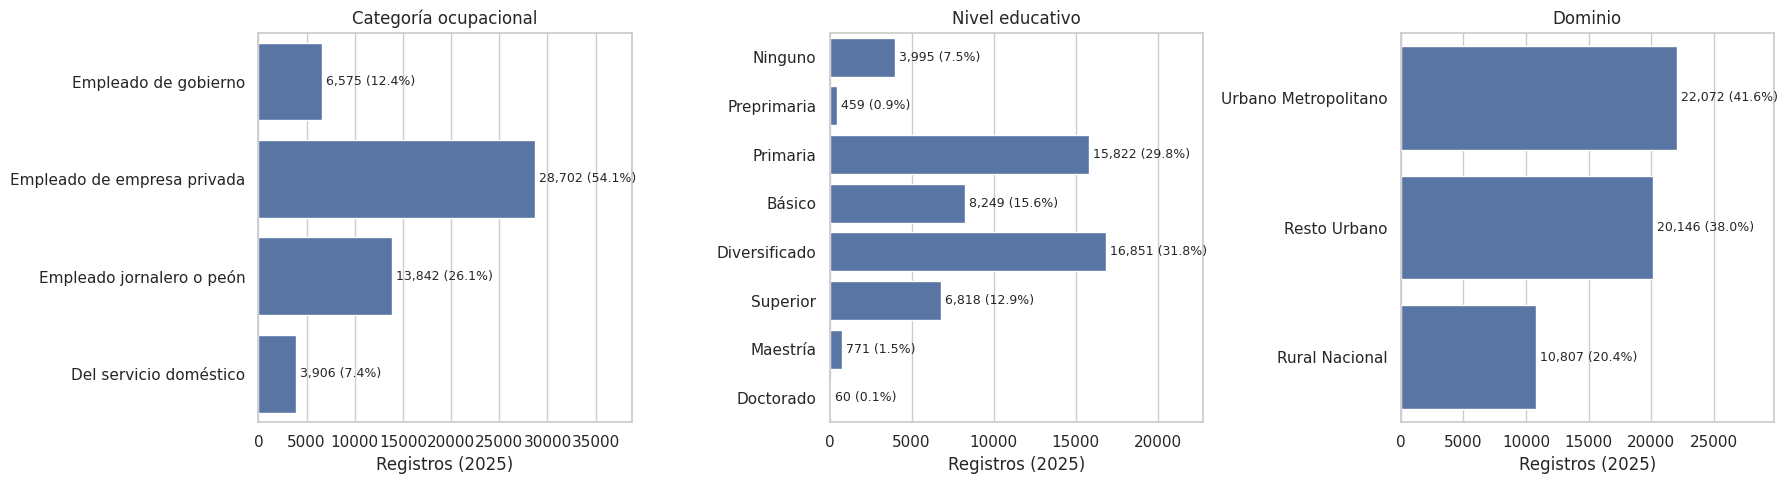
\includegraphics[width=\textwidth]{distribucion_categorias.png}
\caption{Registros de 2025 por categoría ocupacional, nivel educativo y dominio.}
\label{fig:categorias}
\end{figure}

Más de la mitad de los registros son empleados de empresa privada (54.1\,\%), seguidos por jornaleros o peones (26.1\,\%), empleados de gobierno (12.4\,\%) y servicio doméstico (7.4\,\%). En educación predominan diversificado (31.8\,\%) y primaria (29.8\,\%), seguidos de básico (15.6\,\%), superior (12.9\,\%) y ninguno (7.5\,\%). Preprimaria (459 registros), maestría (771) y doctorado (60) son grupos pequeños, y cualquier estadística sobre ellos tiene más incertidumbre. Por dominio, el 41.6\,\% es urbano metropolitano, el 38.0\,\% resto urbano y el 20.4\,\% rural. Estas proporciones describen la muestra sin ponderar.

\subsection{Forma de la distribución del salario}

\begin{figure}[H]
\centering
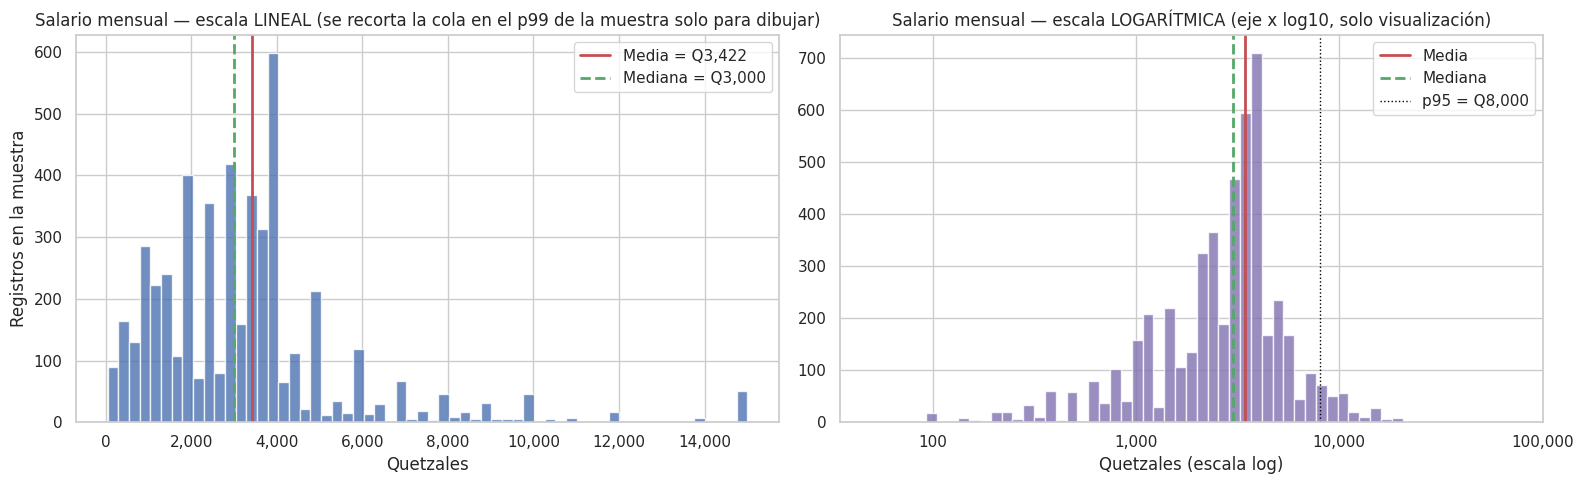
\includegraphics[width=\textwidth]{distribucion_salario.png}
\caption{Salario mensual en escala lineal (izq., cola recortada en el P99 de la muestra solo para dibujar) y en escala logarítmica (der.). Muestra de 5\,000 registros; las líneas de media, mediana y P95 usan las estadísticas del conjunto completo.}
\label{fig:salario}
\end{figure}

\textit{¿El salario presenta una distribución simétrica o asimétrica?} Es fuertemente asimétrico a la derecha (coeficiente 6.00). La mitad central está entre Q1\,800 y Q4\,000, pero la cola se extiende hasta Q99\,000, y hay 119 registros con salarios mayores a tres veces el P95 (más de Q24\,000). El 5\,\% superior concentra el 16.45\,\% de la masa salarial y el 1\,\% superior (por encima de Q15\,000) el 4.78\,\%. En escala logarítmica la distribución se ve aproximadamente simétrica, con picos en cifras redondas (Q3\,000, Q4\,000) propios del salario autorreportado. En el extremo inferior hay salarios de hasta Q1, que siguiendo las instrucciones no se eliminaron.

\textit{¿Qué diferencia existe entre su media y su mediana?} La media es Q3\,421.68 y la mediana Q3\,000, una diferencia de Q421.68 (14.1\,\% sobre la mediana). La cola alta arrastra la media hacia arriba; como referencia, al excluir el 1\,\% superior la media baja a Q3\,281.44. La mediana describe mejor el salario típico. Para el modelado, esta asimetría anticipa que el RMSE será bastante mayor que el MAE y que los salarios altos serán difíciles de estimar.

\subsection{Salario mediano por nivel educativo y categoría ocupacional}

\begin{figure}[H]
\centering
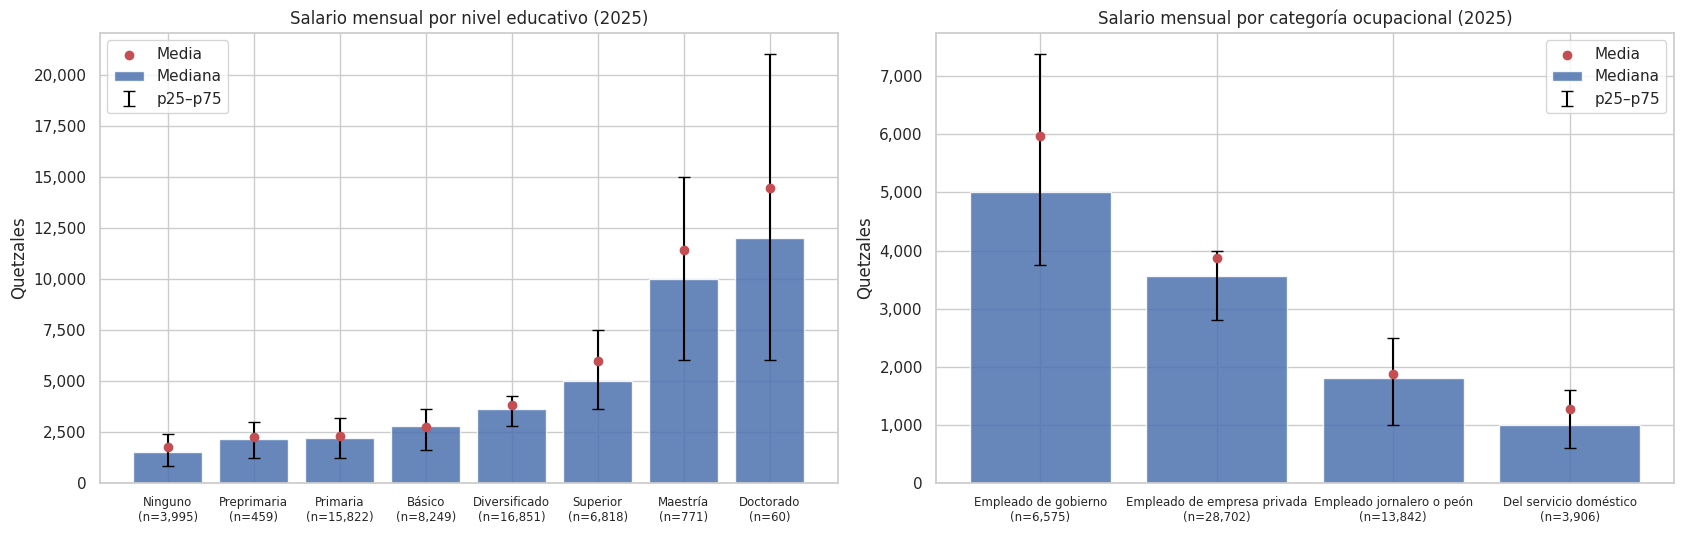
\includegraphics[width=\textwidth]{mediana_edu_cat.png}
\caption{Salario mediano (barras), rango intercuartílico (líneas) y media (puntos) por nivel educativo y por categoría ocupacional, 2025.}
\label{fig:mediana_grupos}
\end{figure}

\begin{table}[H]
\centering
\caption{Salario mensual por nivel educativo y por categoría ocupacional, 2025 (quetzales).}
\label{tab:mediana_grupos}
\small
\begin{tabular}{lrrrrr}
\toprule
Grupo & $n$ & P25 & Mediana & P75 & Media \\
\midrule
Ninguno & 3\,995 & 800 & 1\,500 & 2\,400 & 1\,767 \\
Preprimaria & 459 & 1\,200 & 2\,160 & 3\,000 & 2\,242 \\
Primaria & 15\,822 & 1\,200 & 2\,200 & 3\,200 & 2\,308 \\
Básico & 8\,249 & 1\,600 & 2\,800 & 3\,600 & 2\,730 \\
Diversificado & 16\,851 & 2\,800 & 3\,600 & 4\,250 & 3\,796 \\
Superior & 6\,818 & 3\,600 & 5\,000 & 7\,500 & 5\,965 \\
Maestría & 771 & 6\,000 & 10\,000 & 15\,000 & 11\,409 \\
Doctorado & 60 & 6\,000 & 12\,000 & 21\,000 & 14\,452 \\
\midrule
Empleado de gobierno & 6\,575 & 3\,750 & 5\,000 & 7\,380 & 5\,972 \\
Empleado de empresa privada & 28\,702 & 2\,800 & 3\,568 & 4\,000 & 3\,875 \\
Empleado jornalero o peón & 13\,842 & 1\,000 & 1\,800 & 2\,490 & 1\,879 \\
Servicio doméstico & 3\,906 & 600 & 1\,000 & 1\,600 & 1\,266 \\
\bottomrule
\end{tabular}
\end{table}

\textit{¿Cómo varía el salario mediano entre niveles educativos y categorías ocupacionales?} La mediana crece con cada nivel educativo, de Q1\,500 sin estudios a Q3\,600 con diversificado, Q5\,000 con estudios superiores y Q10\,000 con maestría. El salto más marcado ocurre a partir del nivel superior, y es también donde la dispersión aumenta (el rango intercuartílico de maestría va de Q6\,000 a Q15\,000). Entre categorías, gobierno tiene la mediana más alta (Q5\,000), seguido de empresa privada (Q3\,568), jornaleros (Q1\,800) y servicio doméstico (Q1\,000).

\begin{figure}[H]
\centering
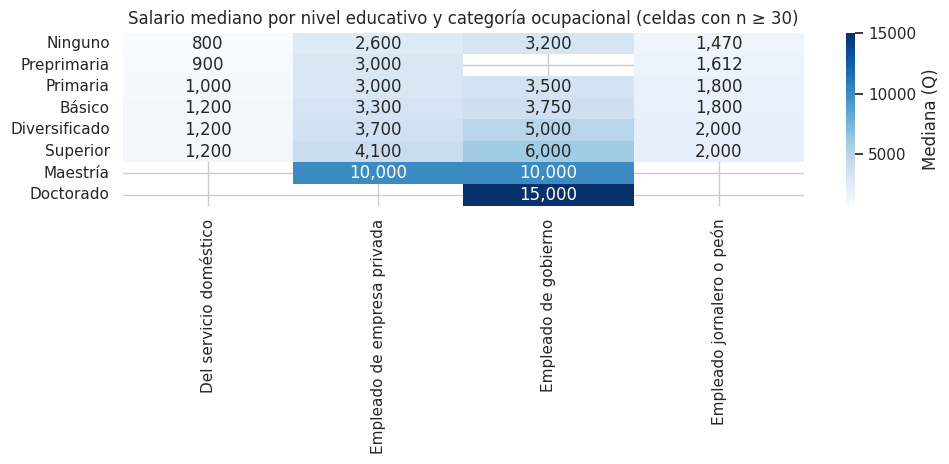
\includegraphics[width=0.8\textwidth]{heatmap_edu_cat.png}
\caption{Salario mediano por nivel educativo y categoría ocupacional (se ocultan celdas con menos de 30 registros).}
\label{fig:heatmap}
\end{figure}

El cruce de ambas variables (Figura~\ref{fig:heatmap}) muestra que la educación y la categoría no actúan igual en todos los grupos. En gobierno y empresa privada la mediana sube claramente con la educación (en gobierno, de Q3\,200 sin estudios a Q6\,000 con superior y Q15\,000 con doctorado). En servicio doméstico y trabajo jornalero casi no cambia: la mediana del servicio doméstico se queda entre Q800 y Q1\,200 y la del jornalero entre Q1\,470 y Q2\,000 en todos los niveles. Esta interacción es relevante para el modelado, porque una regresión lineal con efectos aditivos no puede representarla directamente. La asociación es descriptiva y no implica que la educación cause el salario.

\subsection{Tamaño de la muestra y salario mediano por trimestre}

\begin{figure}[H]
\centering
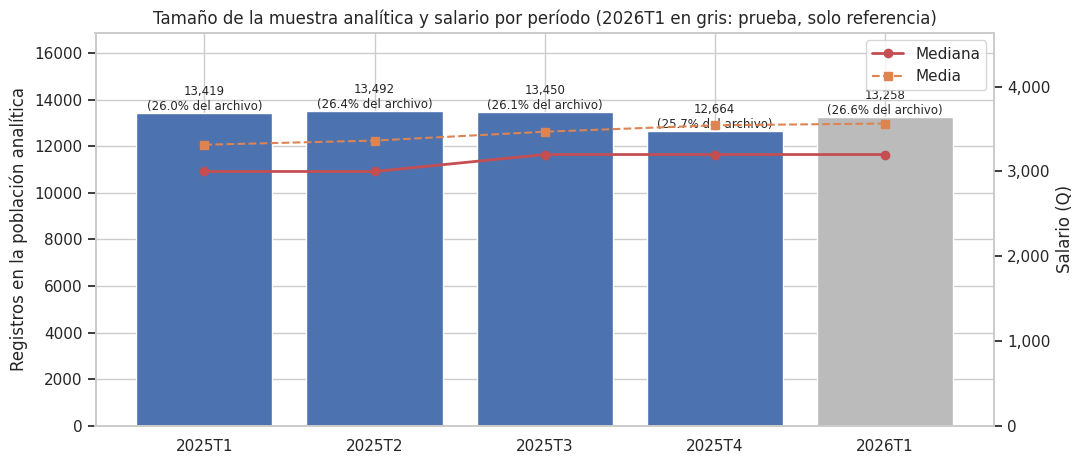
\includegraphics[width=0.85\textwidth]{trimestres.png}
\caption{Registros en la población analítica (barras) y salario mediano y medio (líneas) por período. 2026T1 se muestra en gris solo como referencia.}
\label{fig:trimestres}
\end{figure}

\begin{table}[H]
\centering
\caption{Tamaño de la población analítica y salario por período.}
\label{tab:trimestres}
\small
\begin{tabular}{lrrr}
\toprule
Período & Registros & Mediana (Q) & Media (Q) \\
\midrule
2025T1 & 13\,419 & 3\,000 & 3\,315.63 \\
2025T2 & 13\,492 & 3\,000 & 3\,364.57 \\
2025T3 & 13\,450 & 3\,200 & 3\,469.07 \\
2025T4 & 12\,664 & 3\,200 & 3\,544.57 \\
2026T1 & 13\,258 & 3\,200 & 3\,565.80 \\
\bottomrule
\end{tabular}
\end{table}

\textit{¿Cómo cambian el tamaño de la muestra analítica y el salario mediano entre trimestres?} El tamaño es estable en los tres primeros trimestres (unos 13\,450 registros) y baja a 12\,664 en 2025T4 porque ese archivo trae menos filas; la proporción retenida se mantiene cerca del 26\,\% en todos. La mediana pasa de Q3\,000 en los dos primeros trimestres a Q3\,200 desde el tercero, y la media sube de forma continua de Q3\,315.63 a Q3\,565.80 en 2026T1. Son cifras nominales, sin ajuste por inflación. Esta tendencia importa para el diseño de la validación: un modelo entrenado con trimestres anteriores tenderá a subestimar levemente los salarios de los períodos posteriores.

\section{Relaciones entre variables numéricas}

Las correlaciones se calcularon con \var{VectorAssembler} y con \var{Correlation.corr()} del módulo \var{pyspark.ml.stat}, sobre los 53\,025 registros elegibles de 2025. Se reporta Pearson, la requerida, y Spearman como complemento, dado que el salario es muy asimétrico.

\begin{table}[H]
\centering
\caption{Matriz de correlación de Pearson, 2025 ($n = 53\,025$).}
\label{tab:pearson}
\small
\begin{tabular}{lrrrr}
\toprule
 & Salario & Edad & Antigüedad & Horas \\
\midrule
Salario mensual & 1.000 & 0.147 & 0.180 & 0.076 \\
Edad & 0.147 & 1.000 & 0.487 & $-0.105$ \\
Antigüedad & 0.180 & 0.487 & 1.000 & $-0.062$ \\
Horas semanales & 0.076 & $-0.105$ & $-0.062$ & 1.000 \\
\bottomrule
\end{tabular}
\end{table}

\begin{figure}[H]
\centering
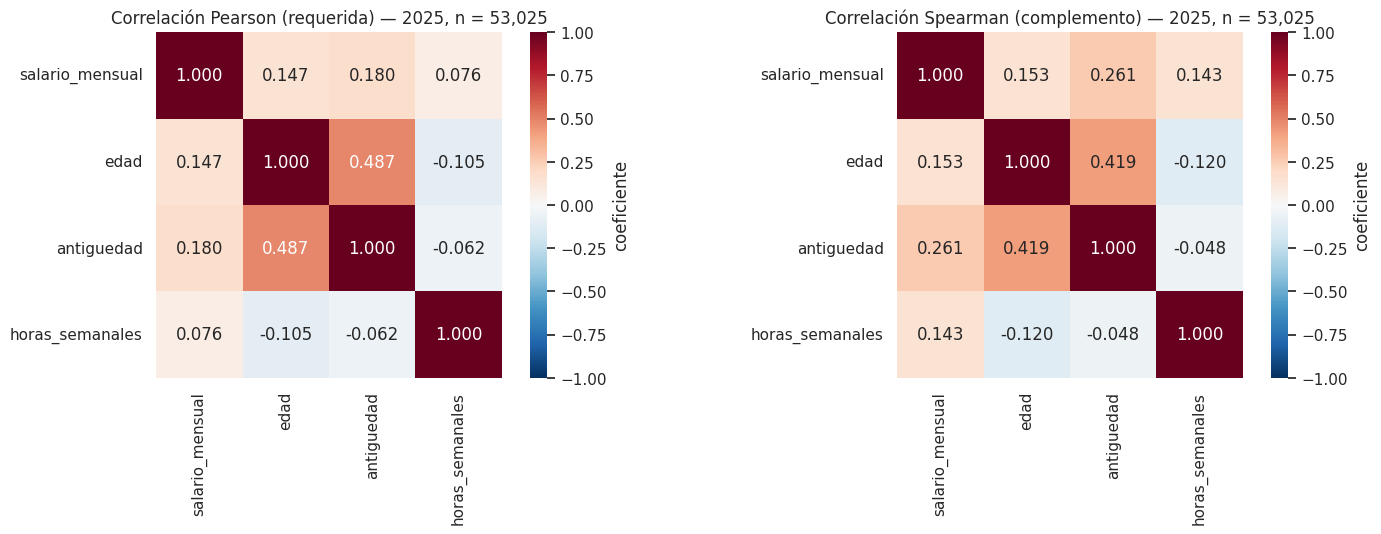
\includegraphics[width=\textwidth]{correlaciones.png}
\caption{Mapas de calor de las correlaciones de Pearson (izq.) y Spearman (der.).}
\label{fig:correlaciones}
\end{figure}

\begin{figure}[H]
\centering
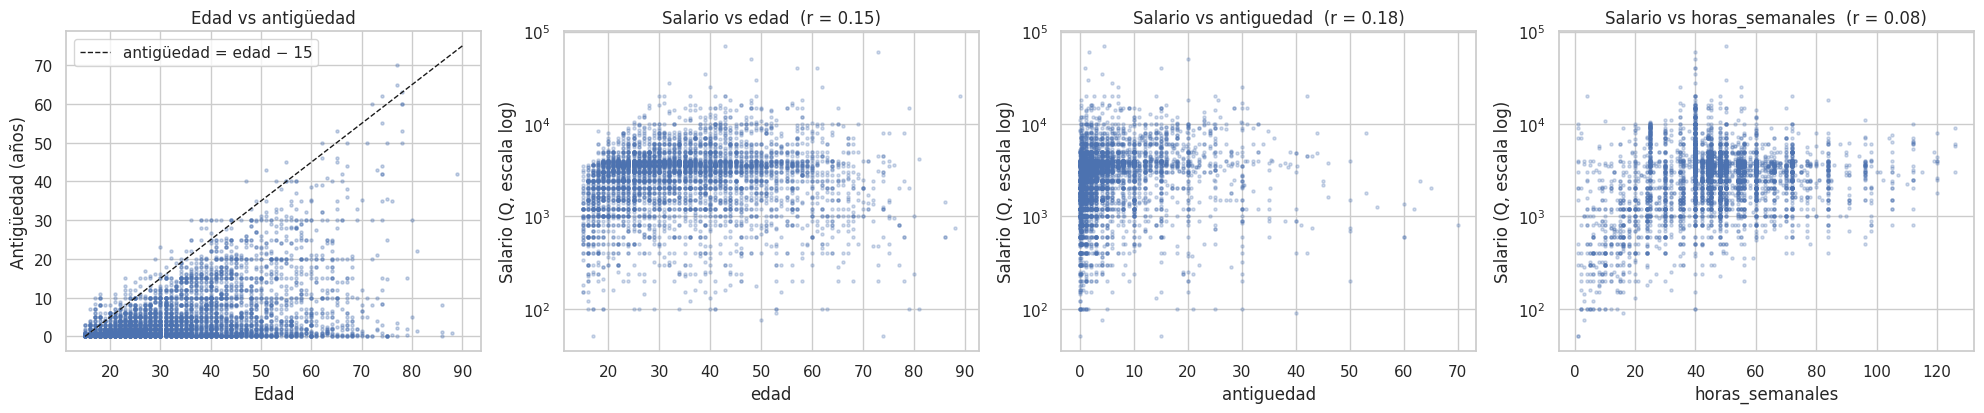
\includegraphics[width=\textwidth]{dispersion_numericas.png}
\caption{Edad frente a antigüedad y salario frente a cada variable numérica (muestra de 5\,000 registros; eje de salario en escala logarítmica).}
\label{fig:dispersion}
\end{figure}

\textit{¿Qué variables presentan mayor asociación lineal con el salario?} La antigüedad (0.180) y la edad (0.147), seguidas de lejos por las horas habituales (0.076). Todas son asociaciones débiles: ninguna de las tres variables numéricas, por sí sola, explica una parte importante de la variación del salario. Con Spearman la antigüedad sube a 0.261 y las horas a 0.143, lo que indica que parte de la relación es monótona pero no lineal, y que Pearson queda atenuado por los salarios extremos. Lo visto en la sección anterior sugiere que la educación y la categoría ocupacional, que no entran en esta matriz, concentran más información sobre el salario.

\textit{¿Existe relación entre edad y antigüedad?} Sí, positiva y moderada (0.487 con Pearson, 0.419 con Spearman). Es esperable porque la antigüedad está acotada por la edad: nadie puede llevar más años en un empleo de los que ha vivido desde que empezó a trabajar, y la Figura~\ref{fig:dispersion} muestra ese límite triangular. No es más fuerte porque muchas personas mayores llevan poco tiempo en su empleo actual. Las horas tienen una relación débil y negativa con la edad ($-0.105$): los más jóvenes reportan jornadas algo más largas.

\section{Segmentación de perfiles mediante KMeans}

\subsection{Variables, estandarización y selección de K}

La segmentación se construyó con un pipeline de \var{VectorAssembler}, \var{StandardScaler} (media 0 y desviación 1) y \var{KMeans} con semilla fija, ajustado sobre los 53\,025 registros de 2025. Se compararon dos conjuntos de variables: el conjunto A, con edad, antigüedad y horas semanales; y el conjunto B, que añade el salario. Para cada uno se probó $K \in \{2, 3, 4, 5\}$ y se registró la silueta (distancia euclidiana cuadrada), el WSSE y el tamaño del cluster más pequeño. Las variables categóricas no se incluyeron en la distancia; se usaron después para describir los perfiles.

\begin{table}[H]
\centering
\caption{Calidad de la segmentación según el conjunto de variables y el número de clusters.}
\label{tab:kmeans}
\footnotesize\setlength{\tabcolsep}{4pt}
\begin{tabular}{llrrrl}
\toprule
Conjunto & $K$ & Silueta & WSSE & Cluster mín. (\%) & Tamaños \\
\midrule
A: edad, antigüedad, horas & 2 & 0.5545 & 106\,717 & 27.5 & 38\,421 / 14\,604 \\
 & 3 & 0.4716 & 83\,608 & 19.1 & 30\,994 / 11\,921 / 10\,110 \\
 & \textbf{4} & \textbf{0.4763} & \textbf{64\,438} & \textbf{12.9} & 24\,511 / 12\,745 / 8\,905 / 6\,864 \\
 & 5 & 0.4838 & 54\,990 & 11.7 & 22\,703 / 11\,018 / 6\,607 / 6\,505 / 6\,192 \\
\midrule
B: A + salario & 2 & 0.5146 & 157\,346 & 27.0 & 38\,694 / 14\,331 \\
 & 3 & 0.3371 & 133\,003 & 16.8 & 27\,368 / 16\,774 / 8\,883 \\
 & 4 & 0.3701 & 113\,557 & 14.3 & 24\,669 / 11\,884 / 8\,910 / 7\,562 \\
 & 5 & 0.4137 & 94\,476 & 3.9 & 24\,240 / 11\,482 / 8\,889 / 6\,325 / 2\,089 \\
\bottomrule
\end{tabular}
\end{table}

\begin{figure}[H]
\centering
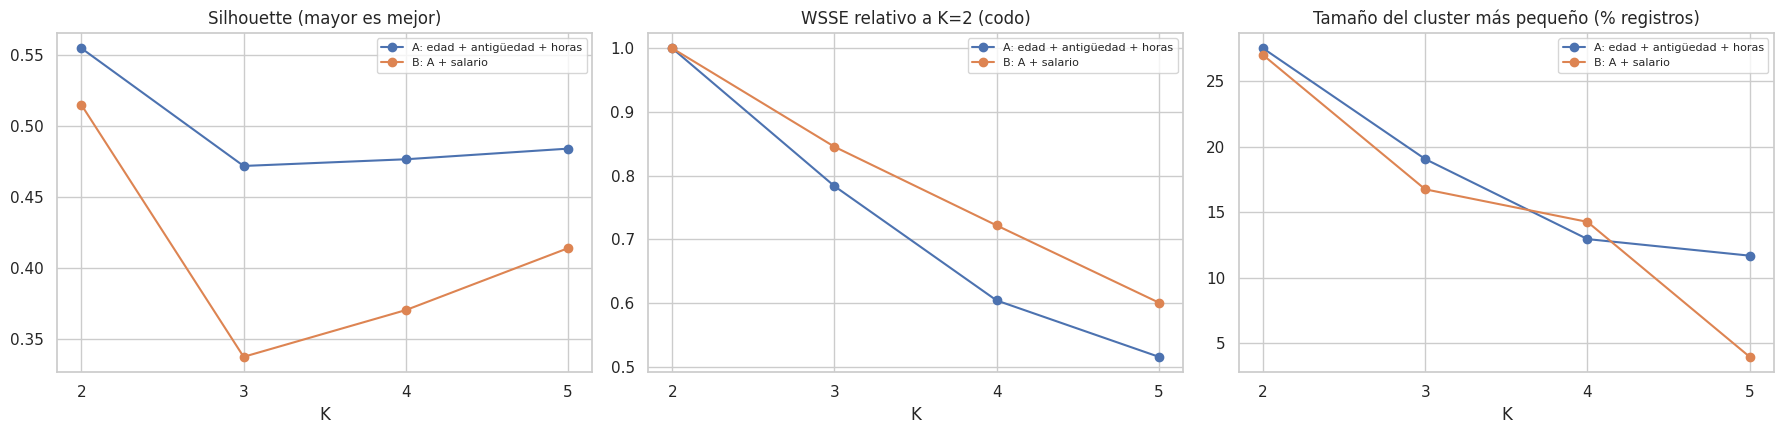
\includegraphics[width=\textwidth]{seleccion_k.png}
\caption{Silueta, WSSE relativo a $K = 2$ y tamaño del cluster más pequeño para ambos conjuntos de variables.}
\label{fig:seleccion_k}
\end{figure}

\textit{¿Vale la pena incluir el salario?} No. Con el salario la silueta es menor para todos los valores de $K$ (por ejemplo, 0.370 frente a 0.476 con $K = 4$), y con $K = 5$ aparece un cluster de apenas el 3.9\,\% de los registros. La cola larga del salario hace que el algoritmo dedique centroides a aislar a quienes ganan mucho en lugar de separar perfiles laborales. Con $K = 2$ el conjunto B se reduce a separar a los mayores de los jóvenes (edad media 50.7 frente a 29.4) con salarios medianos de Q3\,750 y Q3\,000 y salarios máximos de Q99\,000 y Q18\,000, es decir, reproduce la división por edad del conjunto A con más ruido. Además, el salario es la variable que se estima en la segunda parte; segmentar sin él permite usar los clusters para describir cómo varía el salario entre perfiles definidos de forma independiente.

\textit{¿Qué K elegir?} El criterio del grupo combina la silueta, el codo del WSSE y un tamaño mínimo de cluster razonable. $K = 2$ tiene la silueta más alta (0.555), pero solo separa jóvenes de mayores y no distingue la jornada ni la antigüedad. Entre $K = 3$, 4 y 5 las siluetas son parecidas (0.472, 0.476 y 0.484). $K = 4$ captura la mayor reducción del WSSE después de $K = 2$ (de 83\,608 a 64\,438, frente a una reducción menor de 64\,438 a 54\,990 al pasar a $K = 5$) y produce cuatro perfiles interpretables con un cluster mínimo del 12.9\,\%. $K = 5$ gana apenas 0.008 de silueta a cambio de partir perfiles ya definidos en grupos menos distinguibles. Se eligió el conjunto A con $K = 4$. Una silueta de 0.476 indica una estructura moderada: los grupos existen, pero con fronteras que se tocan, como es de esperar en variables continuas sin grupos naturales marcados.

\subsection{Descripción de los perfiles}

\begin{table}[H]
\centering
\caption{Perfil de cada cluster ($K = 4$, conjunto A). El salario, la educación, la categoría y el dominio no participan en la segmentación y se usan solo para describir.}
\label{tab:perfiles}
\small
\begin{tabular}{lrrrr}
\toprule
 & Cluster 0 & Cluster 1 & Cluster 2 & Cluster 3 \\
\midrule
Registros & 12\,745 & 24\,511 & 6\,864 & 8\,905 \\
\% del total & 24.0 & 46.2 & 12.9 & 16.8 \\
Edad media (mediana) & 48.5 (46) & 25.8 (26) & 49.9 (48) & 30.6 (29) \\
Antigüedad media (mediana) & 4.1 (3.0) & 2.4 (1.2) & 22.2 (20.0) & 3.5 (2.0) \\
Horas semanales media (mediana) & 39.4 (42) & 41.0 (44) & 41.1 (40) & 74.8 (72) \\
Salario mediano (Q) & 3\,000 & 3\,000 & 3\,800 & 3\,000 \\
Salario medio (Q) & 3\,535 & 3\,075 & 4\,680 & 3\,244 \\
\% diversificado o más & 37.8 & 51.8 & 49.7 & 40.1 \\
\% rural & 18.1 & 21.8 & 16.7 & 22.5 \\
\% gobierno / privada & 14.1 / 46.3 & 7.8 / 57.2 & 31.4 / 40.4 & 8.0 / 67.4 \\
\% jornalero / doméstico & 27.3 / 12.3 & 29.2 / 5.8 & 22.3 / 5.9 & 18.8 / 5.8 \\
\bottomrule
\end{tabular}
\end{table}

\begin{figure}[H]
\centering
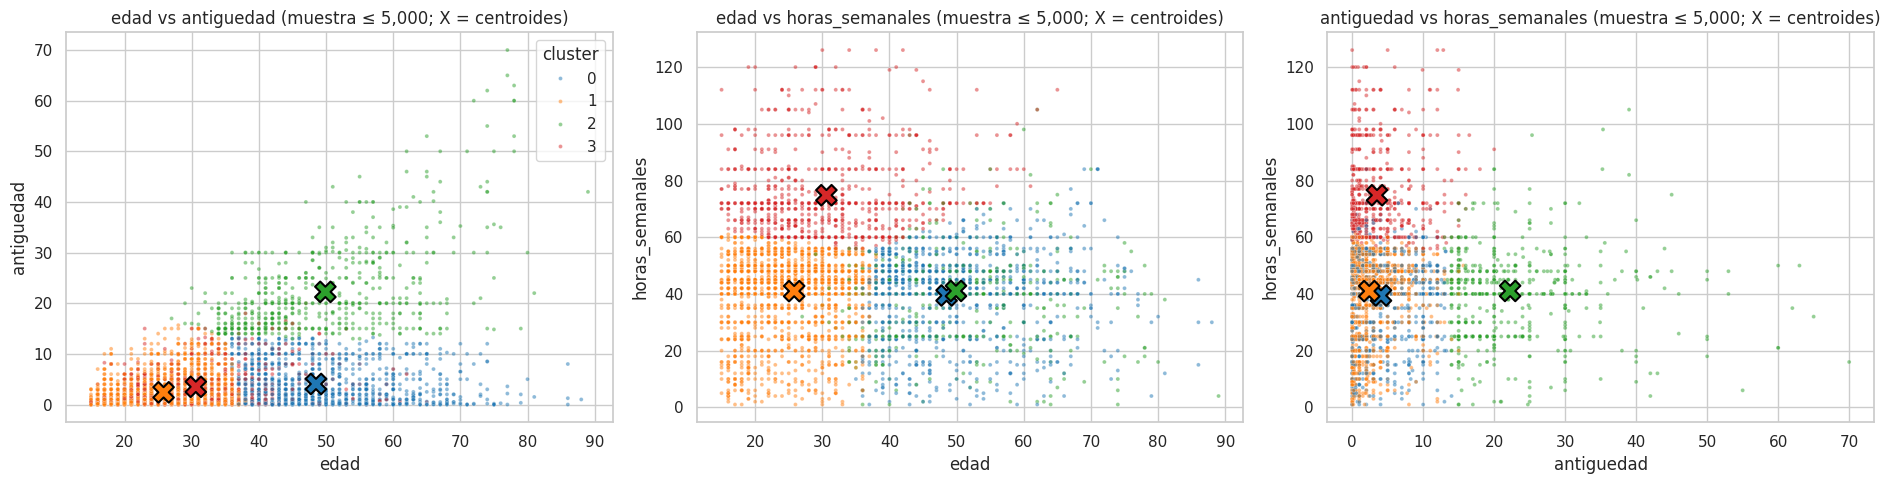
\includegraphics[width=\textwidth]{dispersion_clusters.png}
\caption{Clusters en los tres planos de las variables usadas (muestra de 5\,000 registros; las X marcan los centroides).}
\label{fig:clusters}
\end{figure}

\begin{figure}[H]
\centering
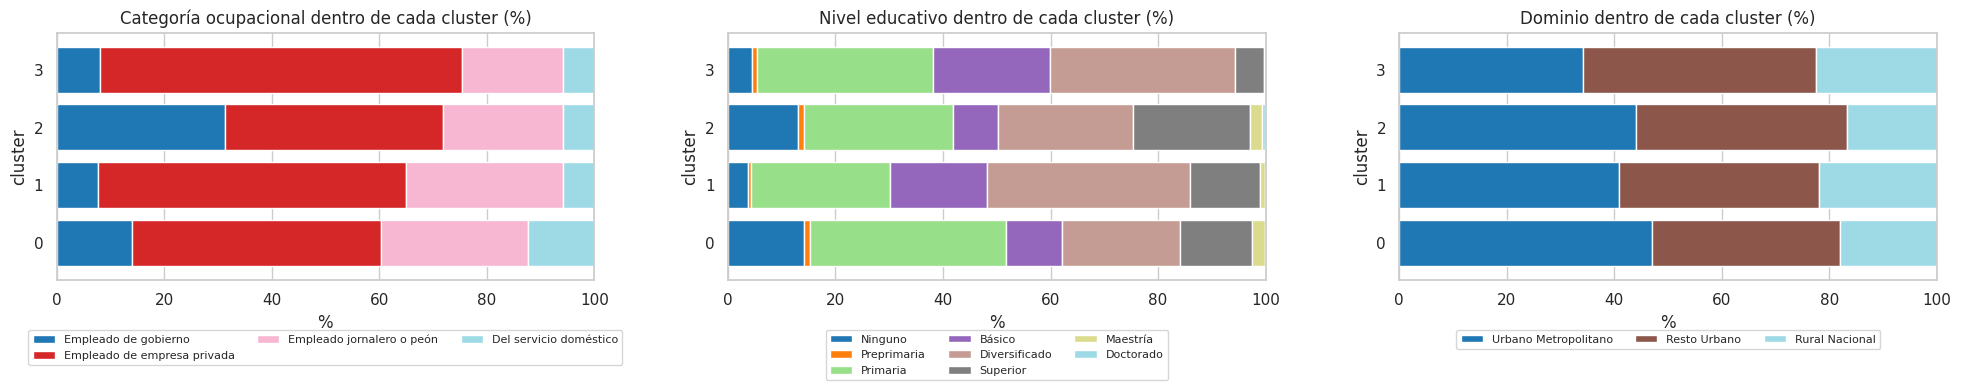
\includegraphics[width=\textwidth]{composicion_clusters.png}
\caption{Composición de cada cluster por categoría ocupacional, nivel educativo y dominio.}
\label{fig:composicion}
\end{figure}

\begin{figure}[H]
\centering
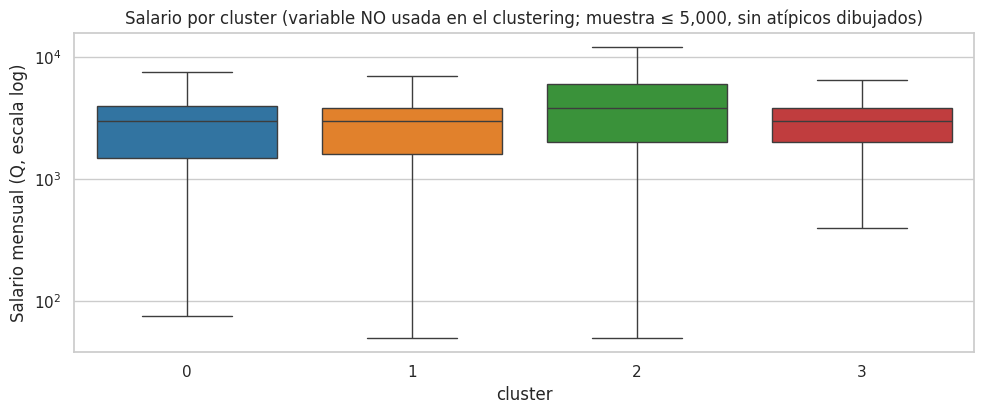
\includegraphics[width=0.75\textwidth]{salario_clusters.png}
\caption{Salario por cluster en escala logarítmica (variable no usada en la segmentación; muestra de 5\,000 registros, sin atípicos dibujados).}
\label{fig:salario_clusters}
\end{figure}

Con base en los centroides y en la composición de cada grupo, los cuatro perfiles se describen así.

\textit{Cluster 1: jóvenes con poca antigüedad y jornada estándar} (46.2\,\%). Es el grupo más numeroso. Edad media de 25.8 años, poco más de un año de antigüedad mediana y unas 41 horas semanales. Es el perfil con mayor proporción de diversificado o más (51.8\,\%) y de empleo privado (57.2\,\%), y tiene el salario medio más bajo (Q3\,075), consistente con personas al inicio de su trayectoria.

\textit{Cluster 0: adultos maduros con empleo reciente} (24.0\,\%). Edad similar a la del cluster 2 (48.5 años) pero con solo 4.1 años de antigüedad media y la jornada más corta (39.4 horas). Es el grupo con menor escolaridad (14.1\,\% sin estudios y 37.8\,\% con diversificado o más) y con la mayor presencia de servicio doméstico (12.3\,\%) y trabajo jornalero (27.3\,\%). Su salario mediano (Q3\,000) es igual al de los jóvenes pese a la diferencia de edad: la edad sin antigüedad acumulada no se asocia con un salario mayor.

\textit{Cluster 2: trabajadores estables de larga trayectoria} (12.9\,\%). Edad media de 49.9 años y 22.2 años de antigüedad, muy por encima del resto (2.13 desviaciones estándar sobre la media en el centroide estandarizado). Concentra el empleo público (31.4\,\% frente a 8\,\% a 14\,\% en los demás) y la mayor proporción de educación superior (21.6\,\%). Es el único grupo con un salario mediano distinto (Q3\,800) y el de mayor salario medio (Q4\,680).

\textit{Cluster 3: jornadas extendidas} (16.8\,\%). Edad media de 30.6 años, antigüedad baja y una jornada habitual de 74.8 horas, unas 34 horas más que los otros grupos. Es el perfil más concentrado en empresa privada (67.4\,\%), con poca educación superior (5.3\,\%) y más presencia fuera del área metropolitana (43.3\,\% resto urbano y 22.5\,\% rural). Su salario mediano es el mismo Q3\,000 de los clusters 0 y 1, lo que implica que obtiene ese salario con casi el doble de horas.

La segmentación muestra que la antigüedad es la variable que mejor se asocia con diferencias de salario entre perfiles, mientras que la edad por sí sola (cluster 0) y las horas (cluster 3) no se traducen en un salario mediano mayor. Las diferencias salariales dentro de cada cluster siguen siendo grandes (Figura~\ref{fig:salario_clusters}), lo que confirma que estas tres variables explican solo una parte del salario.

\section{Diseño del modelado supervisado}

La tarea consiste en estimar \var{salario\_mensual}, en quetzales y sin transformar, con exactamente seis predictores: \var{edad}, \var{antiguedad}, \var{horas\_semanales}, \var{nivel\_educativo}, \var{categoria\_ocupacional} y \var{dominio}. No se usaron identificadores, \var{FACTOR}, otros ingresos, salario por hora ni la etiqueta de cluster. Es una predicción del salario del período observado, no un pronóstico del salario futuro de una persona.

La partición respeta el orden temporal y la indicación del enunciado:

\begin{table}[H]
\centering
\caption{Conjuntos de entrenamiento, validación y prueba.}
\label{tab:particion}
\small
\begin{tabular}{llr}
\toprule
Conjunto & Períodos & Registros \\
\midrule
Entrenamiento (selección de configuración) & 2025T1, 2025T2, 2025T3 & 40\,361 \\
Validación & 2025T4 & 12\,664 \\
Entrenamiento final & 2025T1 a 2025T4 & 53\,025 \\
Prueba final & 2026T1 & 13\,258 \\
\bottomrule
\end{tabular}
\end{table}

Cada pipeline se ajustó completo (indexadores, codificadores, escalado y modelo) solo con los datos de entrenamiento de su etapa, de modo que las categorías y las escalas no se aprenden del conjunto evaluado. El primer trimestre de 2026 no se utilizó hasta la evaluación final. Como modelo de referencia se usó la predicción constante de la media del salario de entrenamiento (Q3\,383 en la etapa de validación, Q3\,421.68 en la evaluación final). Las métricas son MAE, RMSE y $R^2$, calculadas con \var{RegressionEvaluator} sobre todos los registros del conjunto evaluado.

En validación, el modelo de referencia obtiene MAE de Q1\,672.50, RMSE de Q2\,889.57 y $R^2$ de 0.00. El $R^2$ es nulo por construcción, porque una constante no explica varianza; no es exactamente cero porque la media de validación (Q3\,544.57) es mayor que la de entrenamiento. Es el nivel mínimo que cualquier modelo con predictores debe superar.

\section{Pipeline de regresión lineal}

El pipeline incluye \var{StringIndexer} y \var{OneHotEncoder} para las tres variables categóricas, un \var{VectorAssembler} que une las tres numéricas con las categóricas codificadas y un \var{LinearRegression} con la estandarización interna activada (\var{standardization=True}), sin \var{StandardScaler} adicional. Los indexadores usan \var{handleInvalid="keep"} para que una categoría no vista en entrenamiento no interrumpa la predicción. Se probaron cuatro configuraciones de regularización.

\begin{table}[H]
\centering
\caption{Configuraciones de regresión lineal evaluadas en validación (2025T4), ordenadas por RMSE.}
\label{tab:lr}
\small
\begin{tabular}{lrrrrr}
\toprule
Configuración & \var{regParam} & \var{elasticNetParam} & MAE (Q) & RMSE (Q) & $R^2$ \\
\midrule
\textbf{Sin regularización} & \textbf{0.0} & \textbf{0.0} & \textbf{1\,210.14} & \textbf{2\,186.42} & \textbf{0.4257} \\
Ridge (L2) & 0.1 & 0.0 & 1\,210.13 & 2\,186.42 & 0.4257 \\
Elastic net & 0.1 & 0.5 & 1\,210.11 & 2\,186.42 & 0.4257 \\
Lasso (L1) & 0.3 & 1.0 & 1\,210.00 & 2\,186.45 & 0.4257 \\
\bottomrule
\end{tabular}
\end{table}

Las cuatro configuraciones son prácticamente idénticas: el RMSE varía menos de tres centavos. Con seis predictores y más de 40\,000 registros de entrenamiento el modelo tiene muy pocos parámetros en relación con los datos, así que no hay sobreajuste que la penalización pueda corregir, y los valores de \var{regParam} probados apenas mueven los coeficientes estandarizados. Siguiendo el criterio del enunciado se seleccionó la configuración de menor RMSE de validación, la que no usa regularización.

Frente al modelo de referencia, la regresión lineal reduce el MAE en un 27.6\,\% (de Q1\,672.50 a Q1\,210.14) y el RMSE en un 24.3\,\% (de Q2\,889.57 a Q2\,186.42), y explica el 42.6\,\% de la varianza del salario en un trimestre que no vio. Los seis predictores aportan información sustancial, pero más de la mitad de la variación queda sin explicar. El RMSE es 1.8 veces el MAE, efecto directo de la cola de salarios altos: unos pocos errores grandes pesan mucho en el error cuadrático.

\section{Pipeline de Random Forest}

El pipeline repite las etapas de indexación, codificación y ensamblado, y termina en un \var{RandomForestRegressor} con semilla fija, sin estandarización. Se usaron los mismos conjuntos de entrenamiento y validación que en la regresión lineal y se probaron tres combinaciones de número de árboles y profundidad máxima.

\begin{table}[H]
\centering
\caption{Configuraciones de Random Forest evaluadas en validación (2025T4), ordenadas por RMSE.}
\label{tab:rf}
\small
\begin{tabular}{rrrrr}
\toprule
\var{numTrees} & \var{maxDepth} & MAE (Q) & RMSE (Q) & $R^2$ \\
\midrule
\textbf{100} & \textbf{12} & \textbf{1\,060.52} & \textbf{1\,935.91} & \textbf{0.5497} \\
100 & 8 & 1\,096.33 & 2\,028.25 & 0.5058 \\
50 & 5 & 1\,154.51 & 2\,167.92 & 0.4354 \\
\bottomrule
\end{tabular}
\end{table}

El error baja de forma consistente al aumentar la profundidad. Con profundidad 5 el bosque apenas supera a la regresión lineal ($R^2$ de 0.435 frente a 0.426); con profundidad 12 alcanza 0.550. Una mayor profundidad permite más particiones sucesivas y, con ellas, combinaciones más específicas de educación, categoría, antigüedad y horas. Se seleccionó la configuración de 100 árboles y profundidad 12, la de menor RMSE de validación.

\begin{table}[H]
\centering
\caption{Comparación de las configuraciones seleccionadas en validación (2025T4).}
\label{tab:comparacion_val}
\small
\begin{tabular}{lrrr}
\toprule
Modelo & MAE (Q) & RMSE (Q) & $R^2$ \\
\midrule
Referencia (media de entrenamiento) & 1\,672.50 & 2\,889.57 & 0.00 \\
Regresión lineal (sin regularización) & 1\,210.14 & 2\,186.42 & 0.43 \\
Random Forest (100 árboles, prof. 12) & 1\,060.52 & 1\,935.91 & 0.55 \\
\bottomrule
\end{tabular}
\end{table}

\textit{¿Cuál de los dos algoritmos obtuvo mejores resultados en validación y qué diferencias podrían explicar su desempeño?} Random Forest es mejor en las tres métricas: reduce el MAE en un 12.4\,\% y el RMSE en un 11.5\,\% respecto a la regresión lineal, y eleva el $R^2$ de 0.43 a 0.55. Frente a la referencia, reduce el MAE en un 36.6\,\% y el RMSE en un 33.0\,\%. La diferencia es coherente con lo observado en la exploración. La regresión lineal suma un efecto fijo por cada predictor, de modo que el aumento asociado a pasar de primaria a superior es el mismo para un jornalero que para un empleado de gobierno; la Figura~\ref{fig:heatmap} muestra que en realidad ese aumento es grande en gobierno y empresa privada y casi nulo en servicio doméstico y trabajo jornalero. Los árboles representan esas interacciones de forma natural al partir primero por una variable y luego por otra. Además, la relación entre salario y antigüedad o edad no es lineal (la correlación de Spearman supera a la de Pearson), y los árboles la aproximan por tramos sin suponer una forma funcional. La regresión lineal conserva la ventaja de ser directamente interpretable.

\section{Entrenamiento final y evaluación en 2026}

Con una configuración seleccionada por algoritmo, ambos pipelines se reentrenaron con los cuatro trimestres de 2025 (53\,025 registros) y se aplicaron sobre el conjunto de 2026T1, preparado con las mismas reglas de armonización, filtrado y etiquetado. Los tres modelos se evaluaron sobre exactamente los mismos 13\,258 registros elegibles.

\begin{table}[H]
\centering
\caption{Evaluación final en el primer trimestre de 2026 ($n = 13\,258$).}
\label{tab:test}
\small
\begin{tabular}{lrrr}
\toprule
Modelo & MAE (Q) & RMSE (Q) & $R^2$ \\
\midrule
Referencia (media de 2025) & 1\,718.09 & 2\,871.42 & 0.00 \\
Regresión lineal & 1\,240.71 & 2\,163.75 & 0.43 \\
Random Forest & 1\,088.34 & 1\,924.87 & 0.55 \\
\bottomrule
\end{tabular}
\end{table}

El orden de validación se mantiene en prueba. Random Forest reduce el MAE en un 36.7\,\% y el RMSE en un 33.0\,\% frente a la referencia, y en un 12.3\,\% y un 11.0\,\% frente a la regresión lineal. Las métricas de prueba son muy parecidas a las de validación: el MAE sube unos Q30 en ambos modelos, el RMSE baja entre Q11 y Q23 y el $R^2$ se mantiene en 0.43 y 0.55. Ninguno de los dos modelos muestra pérdida de desempeño al pasar a un trimestre nunca visto, lo que indica que la configuración elegida en 2025T4 no quedó sobreajustada a ese período. El leve aumento del MAE es consistente con el alza del salario nominal entre períodos: la media de 2026T1 (Q3\,565.80) es mayor que la de 2025 (Q3\,421.68), y los modelos, entrenados con 2025, no pueden anticipar ese desplazamiento.

\section{Visualización y análisis de errores}

El residuo se define como salario real menos salario predicho, de modo que un residuo positivo indica subestimación y uno negativo, sobreestimación. Los gráficos usan la misma muestra de 5\,000 registros de prueba para ambos modelos; las métricas por grupo usan los 13\,258 registros.

\begin{figure}[H]
\centering
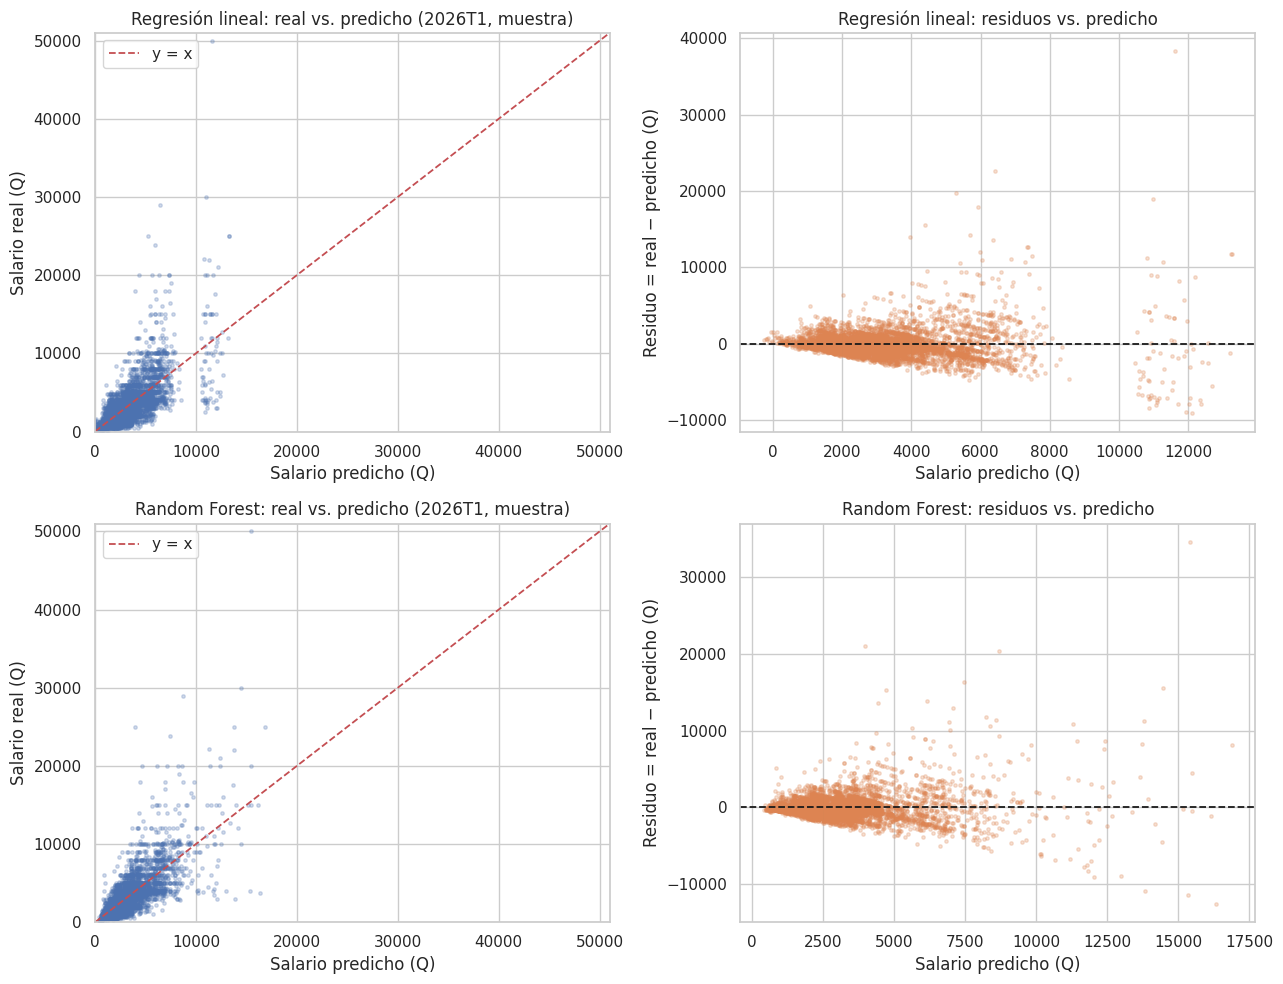
\includegraphics[width=0.95\textwidth]{residuos.png}
\caption{Salario real frente a predicho con la línea $y = x$ (izq.) y residuos frente al salario predicho con la línea en cero (der.), para la regresión lineal (arriba) y Random Forest (abajo). 2026T1, muestra de 5\,000 registros.}
\label{fig:residuos}
\end{figure}

En los dos modelos la nube de real frente a predicho se concentra bajo los Q10\,000 y se abre hacia arriba de la línea $y = x$: hay muchas personas con salarios reales de Q15\,000 a Q50\,000 a quienes los modelos asignan predicciones de Q5\,000 a Q15\,000. Ningún modelo predice valores cercanos a los salarios más altos. Los gráficos de residuos tienen forma de embudo: la dispersión crece con el salario predicho, lo que indica heterocedasticidad. En la parte baja se observa un borde diagonal inferior, porque el salario real no puede ser menor que cero y el residuo más negativo posible es igual a menos la predicción.

Los dos modelos difieren en la forma. La regresión lineal produce un grupo separado de predicciones entre Q10\,000 y Q13\,000, con residuos mayormente negativos: es el efecto aditivo de sumar los coeficientes de educación de posgrado, empleo público y dominio metropolitano, que sobreestima a parte de esas personas. También genera algunas predicciones cercanas a cero, por debajo de cualquier salario plausible. Random Forest distribuye sus predicciones de forma más continua hasta unos Q17\,000 y no produce valores cercanos a cero, porque cada predicción es un promedio de salarios observados en entrenamiento.

\subsection{Errores según el nivel del salario}

\begin{table}[H]
\centering
\caption{Error medio y MAE para los salarios iguales o mayores al P90 de prueba (Q6\,000) y para el resto (quetzales).}
\label{tab:percentil}
\small
\begin{tabular}{lrrrrrr}
\toprule
 & \multicolumn{3}{c}{Salario $\geq$ Q6\,000} & \multicolumn{3}{c}{Salario $<$ Q6\,000} \\
\cmidrule(lr){2-4}\cmidrule(lr){5-7}
Modelo & $n$ & Error medio & MAE & $n$ & Error medio & MAE \\
\midrule
Regresión lineal & 1\,542 & 3\,191.8 & 3\,577.1 & 11\,716 & $-283.7$ & 933.2 \\
Random Forest & 1\,542 & 2\,760.3 & 3\,184.9 & 11\,716 & $-239.9$ & 812.4 \\
\bottomrule
\end{tabular}
\end{table}

El P90 del salario en prueba es Q6\,000. Por la concentración de salarios en cifras redondas, 1\,542 registros (11.6\,\%) quedan en o por encima de ese valor. En ese grupo el error medio es fuertemente positivo en ambos modelos: la regresión lineal subestima en promedio Q3\,192 y Random Forest Q2\,760. Además, en ese grupo el error medio es casi tan grande como el MAE (3\,192 frente a 3\,577, y 2\,760 frente a 3\,185), lo que significa que casi todos los errores tienen el mismo signo. En el 88.4\,\% restante ocurre lo contrario: el error medio es negativo ($-$Q284 y $-$Q240), una sobreestimación leve, y el MAE baja a Q933 y Q812.

Los errores son, por lo tanto, sistemáticos y dependen del nivel del salario. Ambos modelos comprimen las predicciones hacia el centro de la distribución: sobreestiman ligeramente la mayoría de salarios bajos y medios y subestiman de forma marcada los altos. Es el comportamiento esperado de modelos que minimizan el error cuadrático sobre una variable con cola larga, cuando los predictores disponibles no permiten distinguir quién, dentro de un mismo perfil, gana mucho más que el resto. Random Forest atenúa la subestimación de la cola alta en unos Q430, pero no la elimina.

\subsection{Errores por nivel educativo y dominio}

\begin{table}[H]
\centering
\caption{MAE y error medio por nivel educativo en 2026T1 (quetzales).}
\label{tab:error_edu}
\small
\begin{tabular}{lrrrrr}
\toprule
 & & \multicolumn{2}{c}{Regresión lineal} & \multicolumn{2}{c}{Random Forest} \\
\cmidrule(lr){3-4}\cmidrule(lr){5-6}
Nivel educativo & $n$ & MAE & Error medio & MAE & Error medio \\
\midrule
Ninguno & 1\,016 & 823.5 & 109.3 & 633.5 & 20.0 \\
Preprimaria & 80 & 735.2 & 88.8 & 600.7 & $-62.2$ \\
Primaria & 3\,957 & 870.0 & 54.6 & 750.6 & 54.0 \\
Básico & 2\,164 & 894.5 & 127.8 & 809.5 & 139.4 \\
Diversificado & 4\,117 & 1\,109.3 & 104.0 & 1\,013.6 & 111.3 \\
Superior & 1\,729 & 2\,566.4 & 295.5 & 2\,254.1 & 264.7 \\
Maestría & 183 & 5\,552.9 & $-131.5$ & 4\,501.9 & $-340.2$ \\
Doctorado & 12 & 12\,919.3 & 6\,062.7 & 10\,100.7 & 5\,079.9 \\
\bottomrule
\end{tabular}
\end{table}

\begin{table}[H]
\centering
\caption{MAE y error medio por dominio en 2026T1 (quetzales).}
\label{tab:error_dom}
\small
\begin{tabular}{lrrrrr}
\toprule
 & & \multicolumn{2}{c}{Regresión lineal} & \multicolumn{2}{c}{Random Forest} \\
\cmidrule(lr){3-4}\cmidrule(lr){5-6}
Dominio & $n$ & MAE & Error medio & MAE & Error medio \\
\midrule
Urbano Metropolitano & 5\,632 & 1\,446.1 & 136.0 & 1\,303.6 & 158.0 \\
Resto Urbano & 4\,846 & 1\,189.6 & 134.3 & 1\,027.1 & 93.7 \\
Rural Nacional & 2\,780 & 913.6 & 65.2 & 759.1 & 36.5 \\
\bottomrule
\end{tabular}
\end{table}

El MAE crece con el nivel educativo en ambos modelos, siguiendo la dispersión del salario de cada grupo. En los niveles con más observaciones (ninguno a diversificado, el 85\,\% de la prueba) el MAE está entre Q600 y Q1\,110 y el error medio es pequeño. En superior se duplica (Q2\,254 a Q2\,566) y en maestría llega a Q4\,500 a Q5\,550, aunque con un error medio cercano a cero: en maestría los modelos se equivocan mucho en ambas direcciones, sobreestimando a unos y subestimando a otros, porque el rango de salarios del grupo es muy amplio. El doctorado tiene los errores más altos y una subestimación media de Q5\,000 a Q6\,000, pero con solo 12 registros de prueba ese resultado no es confiable. Random Forest tiene menor MAE que la regresión lineal en todos los niveles educativos.

Por dominio, el error es mayor en el área urbana metropolitana (MAE de Q1\,304 a Q1\,446) y menor en el área rural (Q759 a Q914), en línea con que los salarios altos y la mayor dispersión se concentran en la ciudad. En los tres dominios el error medio es positivo: ambos modelos subestiman en promedio los salarios de 2026T1. El error medio global, ponderado por el tamaño de cada dominio, es de unos Q120 en la regresión lineal y Q109 en Random Forest, del mismo orden que el aumento de la media salarial entre 2025 y 2026T1 (Q144). Buena parte de ese sesgo se explica por el desplazamiento nominal de los salarios y no por un defecto particular de los modelos.

\section{Discusión final}

La primera pregunta del laboratorio se responde con cuatro perfiles de asalariados definidos por edad, antigüedad y jornada: jóvenes con poca antigüedad (46\,\%), adultos maduros con empleo reciente (24\,\%), trabajadores de larga trayectoria (13\,\%) y trabajadores con jornadas extendidas (17\,\%). La segmentación tiene una estructura moderada (silueta de 0.476) y solo el perfil de larga trayectoria, más ligado al empleo público y a la educación superior, se distingue por un salario mediano mayor. Incluir el salario en la segmentación la empeoraba y la desviaba hacia aislar la cola de salarios altos.

La segunda pregunta tiene una respuesta cuantitativa: con seis características personales y laborales, el salario mensual de 2026T1 puede estimarse con un error absoluto medio de unos Q1\,090 y un $R^2$ de 0.55 usando Random Forest, frente a Q1\,240 y 0.43 con regresión lineal y Q1\,720 con la media como predicción. Ambos modelos superan con holgura a la referencia y mantienen su desempeño de validación en un trimestre nuevo. La ventaja de Random Forest proviene de su capacidad para representar interacciones, como la de nivel educativo y categoría ocupacional, que la exploración mostró de forma directa.

El límite de ambos modelos está en la cola de la distribución. El salario es muy asimétrico (media de Q3\,422 frente a mediana de Q3\,000, máximo de Q99\,000) y las variables numéricas se asocian débilmente con él (correlaciones de 0.08 a 0.18). Los modelos predicen bien el salario típico, pero subestiman de forma sistemática a quienes ganan Q6\,000 o más, en promedio entre Q2\,760 y Q3\,190, y sobreestiman levemente al resto. Esa subestimación es mayor en los niveles educativos altos y en el área metropolitana, que es donde se concentran esos salarios. Probablemente dependen de variables que no forman parte del conjunto de predictores, como la ocupación específica, el sector económico o el tamaño de la empresa. Una transformación logarítmica del objetivo o una función de pérdida más robusta podrían reducir el peso de la cola, pero quedaron fuera de la comparación obligatoria por instrucción del enunciado, y los salarios extremos se mantuvieron en la evaluación.

Estos resultados describen los registros analizados, sin ponderar por \var{FACTOR}, y no son estimaciones de la población asalariada del país. Las relaciones encontradas entre educación, categoría ocupacional, antigüedad y salario son asociaciones y no demuestran causalidad, y las predicciones no deben interpretarse como el salario que una persona debería recibir.

\section*{Reproducibilidad}

El análisis completo está en el notebook \texttt{Laboratorio7\_SparkMLlib.ipynb}, que se ejecuta de principio a fin sin depender de variables creadas manualmente. Requiere Python con Spark 3.5.x (se usó 3.5.1 con Java 21), pandas, openpyxl, numpy, matplotlib y seaborn. Los archivos originales del INE se colocan en \texttt{data/raw} y sus diccionarios en \texttt{data/diccionarios}; el notebook genera los Parquet crudos por archivo, los conjuntos preparados \texttt{eneic\_2025\_preparado} y \texttt{eneic\_2026\_preparado}, las etiquetas de segmentación y el modelo KMeans guardado. Se usó semilla fija (\texttt{seed=42}) en KMeans, Random Forest y todas las muestras para graficar. Repositorio: \url{\repo}.

\begin{thebibliography}{9}
\bibitem{ine} Instituto Nacional de Estadística de Guatemala. Encuesta Nacional de Empleo e Ingresos Continua (ENEIC), bases de Personas 2025 y 2026. \url{https://www.ine.gob.gt/encuesta-nacional-de-empleo-e-ingresos/}
\bibitem{spark} Apache Software Foundation. MLlib: Main Guide, Apache Spark 3.5. \url{https://spark.apache.org/docs/3.5.1/ml-guide.html}
\bibitem{breiman} Breiman, L. (2001). Random Forests. \textit{Machine Learning}, 45(1), 5--32.
\bibitem{rousseeuw} Rousseeuw, P. J. (1987). Silhouettes: a graphical aid to the interpretation and validation of cluster analysis. \textit{Journal of Computational and Applied Mathematics}, 20, 53--65.
\end{thebibliography}

\end{document}
